\documentclass[]{elsarticle} %review=doublespace preprint=single 5p=2 column
%%% Begin My package additions %%%%%%%%%%%%%%%%%%%
\usepackage[hyphens]{url}
\usepackage{lineno} % add
\providecommand{\tightlist}{%
  \setlength{\itemsep}{0pt}\setlength{\parskip}{0pt}}

\bibliographystyle{elsarticle-harv}
\biboptions{sort&compress} % For natbib
\usepackage{graphicx}
\usepackage{booktabs} % book-quality tables
%% Redefines the elsarticle footer
%\makeatletter
%\def\ps@pprintTitle{%
% \let\@oddhead\@empty
% \let\@evenhead\@empty
% \def\@oddfoot{\it \hfill\today}%
% \let\@evenfoot\@oddfoot}
%\makeatother

% A modified page layout
\textwidth 6.75in
\oddsidemargin -0.15in
\evensidemargin -0.15in
\textheight 9in
\topmargin -0.5in
%%%%%%%%%%%%%%%% end my additions to header

\usepackage[T1]{fontenc}
\usepackage{lmodern}
\usepackage{amssymb,amsmath}
\usepackage{ifxetex,ifluatex}
\usepackage{fixltx2e} % provides \textsubscript
% use upquote if available, for straight quotes in verbatim environments
\IfFileExists{upquote.sty}{\usepackage{upquote}}{}
\ifnum 0\ifxetex 1\fi\ifluatex 1\fi=0 % if pdftex
  \usepackage[utf8]{inputenc}
\else % if luatex or xelatex
  \usepackage{fontspec}
  \ifxetex
    \usepackage{xltxtra,xunicode}
  \fi
  \defaultfontfeatures{Mapping=tex-text,Scale=MatchLowercase}
  \newcommand{\euro}{€}
\fi
% use microtype if available
\IfFileExists{microtype.sty}{\usepackage{microtype}}{}
\usepackage{graphicx}
% We will generate all images so they have a width \maxwidth. This means
% that they will get their normal width if they fit onto the page, but
% are scaled down if they would overflow the margins.
\makeatletter
\def\maxwidth{\ifdim\Gin@nat@width>\linewidth\linewidth
\else\Gin@nat@width\fi}
\makeatother
\let\Oldincludegraphics\includegraphics
\renewcommand{\includegraphics}[1]{\Oldincludegraphics[width=\maxwidth]{#1}}
\ifxetex
  \usepackage[setpagesize=false, % page size defined by xetex
              unicode=false, % unicode breaks when used with xetex
              xetex]{hyperref}
\else
  \usepackage[unicode=true]{hyperref}
\fi
\hypersetup{breaklinks=true,
            bookmarks=true,
            pdfauthor={},
            pdftitle={Assessing exposure to Atlantic Basin tropical storms in United States counties},
            colorlinks=true,
            urlcolor=blue,
            linkcolor=magenta,
            pdfborder={0 0 0}}
\urlstyle{same}  % don't use monospace font for urls
\setlength{\parindent}{0pt}
\setlength{\parskip}{6pt plus 2pt minus 1pt}
\setlength{\emergencystretch}{3em}  % prevent overfull lines
\setcounter{secnumdepth}{0}
% Pandoc toggle for numbering sections (defaults to be off)
\setcounter{secnumdepth}{0}
% Pandoc header


\usepackage[nomarkers]{endfloat}

\begin{document}
\begin{frontmatter}

  \title{Assessing exposure to Atlantic Basin tropical storms in United States
counties}
    \author[Colorado State University]{Joshua Ferreri}
   \ead{joshua.m.ferreri@gmail.com} 
  
    \author[Colorado State University]{Meilin Yan}
   \ead{alice@example.com} 
  
    \author[NASA Marshall Space Flight Center]{Mohammad Z. Al-Hamdan}
   \ead{alice@example.com} 
  
    \author[NASA Marshall Space Flight Center]{William L. Crosson}
   \ead{alice@example.com} 
  
    \author[University of Michigan]{Seth Guikema}
   \ead{alice@example.com} 
  
    \author[Johns Hopkins Bloomberg School of Public Health]{Roger D. Peng}
   \ead{alice@example.com} 
  
    \author[Colorado State University]{G. Brooke Anderson\corref{c1}}
   \ead{brooke.anderson@colostate.edu} 
   \cortext[c1]{Corresponding Author}
      \address[Colorado State University]{Department of Environmental and Radiological Health Sciences, Lake
Street, Fort Collins, CO, Zip}
    \address[NASA Marshall Space Flight Center]{Universities Space Research Association, Street, Huntsville, AL, Zip}
    \address[University of Michigan]{Department, Street, City, State, Zip}
    \address[Johns Hopkins Bloomberg School of Public Health]{Department of Biostatistics, Street, Baltimore, MD, Zip}
  
  \begin{abstract}
  There are many important applications for having county-level estimates
  of exposure to tropical storms over many years. For example, \ldots{} .
  Current approaches include \ldots{} but have the following limitations
  \ldots{} .
  
  Here, we present open source software we have developed to explore
  county-level exposure to tropical storms in United States counties
  between 1988 and 2011. Further, we explore the differences in exposure
  classification when using different metrics (e.g., wind speed, rainfall,
  distance).
  \end{abstract}
  
 \end{frontmatter}

\section{Introduction}\label{introduction}

\paragraph{What it means to assess county-level tropical storm
exposure}\label{what-it-means-to-assess-county-level-tropical-storm-exposure}

\paragraph{Why it's important to measure TS exposure for
counties}\label{why-its-important-to-measure-ts-exposure-for-counties}

Many outcomes of interest are available at county-level aggregations
(e.g., counts of health outcomes: Grabich et al. (2016): premature
births and low birth weights). Further, decisions and policies to
prepare for and respond to storms are often undertaken at the county
level (Zandbergen 2009). Some studies suggest methods to determine
exposure, including inland exposure, to tropical storms at the
county-level over many years (Zandbergen 2009). Here, we offer tools,
through the open-source \texttt{hurricaneexposure} package, to determine
county-level exposure to tropical storms using several different metrics
(distance, rainfall, wind). In this paper, we describe how this software
package assesses exposure to tropical storms at the county level,
provide an analysis of the advantages and disadvantages of different
strategies for assessing county-level exposure, and explore variation in
exposure assessments based on using different exposure metrics.

Current hurricane exposure assignments are often nonspecific {[}GBA-- I
found this wording a bit unclear{]} and may lead to missclassification
of exposure at the county-level (Grabich et al. 2016). Researchers have
found heterogeneity in exposure assignments of counties, both within and
between storms, when different metrics of exposure are used (Grabich et
al. 2016). Such missclassification can have important implications of
assessments of the public health and economic impacts of tropical
storms.

Many of the studies that have assessed exposure to tropical storms in
the US have used geographical information system software (e.g., ArcGIS)
{[}example studies{]}. Here, we offer methods to map and output historic
exposure to tropical storms that does not require the use of proprietary
software but instead uses a package written in the R statistical
programming language, which is free and open-source.

\paragraph{Examples of estimating TS for multiple
storms}\label{examples-of-estimating-ts-for-multiple-storms}

When assessing exposure to a single tropical storm, a detailed analysis
of \ldots{} can be performed for the storm. However, this level of
detailed analysis is unreasonable when assessing exposure to all storms
over an extended time period; further, such a long-term exposure
assessment requires consistency in the data being used to determine
levels of exposure to factors like wind and rain.

A few studies have sought to determine exposure to tropical storms over
a study period that includes multiple storms. For example, \ldots{}
assessed the exposure of counties in Florida to hurricanes during the
2004 season {[}citation{]}. The largest county-level exposure study is
likely that of Zandbergen (2009), which estimated exposure in US
counties to all {[}US landfalling? or all storms?{]} Atlantic basin
tropical storms between 1851 and 2003, using both distance and an
exposure metric that incorporated distance and windspeed. They used this
exposure evaluation to create maps of total exposure to tropical storms
within US counties, as well as to explore associations between a
county's long-term exposure to tropical storms and its location,
distance from the coast, size, and shape (Zandbergen 2009).

\paragraph{Examples of other datasets at the county
level}\label{examples-of-other-datasets-at-the-county-level}

If exposure to tropical storms over multiple storms and years can be
assessed, these exposure datasets can be joined with other time series
to explore the impacts of tropical storms. For example, daily counts of
human health outcomes in environmental epidemiology studies are often
available aggregated at the county level, and such data has often been
paired with time series of environmental exposures (e.g., air pollution,
temperature) to determine associated risks.

\section{Data and Methods}\label{data-and-methods}

\paragraph{Distance-based exposure}\label{distance-based-exposure}

We collected ``best tracks'' data on hurricane tracks for Atlantic basin
storms between 1988 and 2014 from the extended best tracks database.
This dataset is based on a poststorm assessment of each storm conducted
by the United States National Hurricane Center (NHC) and incorporates
data from a variety of sources, including satellite data and, when
available, aircraft reconnaisance data (Landsea and Franklin 2013). This
data gives time stamps for each observation in Coordinated Universal
Time (UTC; also known as Zulu Time, sometimes indicated by ``Z'').

These data typically give measurements of storm center location at
6-hour intervals, at synoptic times (i.e., 6:00 am, 12:00 pm, 6:00 pm,
and 12:00 am UTC); some landfalling storms have an additional
observation at the time of landfall (Landsea and Franklin 2013). These
positions are given to within 0.1 degrees latitude / longitude at these
synoptic times (Landsea and Franklin 2013). We interpolated these
location values to every 15 minutes during the period when the storm was
active, using a linear interpolation between each measured point.

We calculated the distance between each county's center and each of the
15-minute-interval estimates of a storm's location. To do this, we used
the Great Circle method to calculate the distance between pairs of
latitude and longitude coordinates, using the R package \texttt{sp}. For
each county, we used the population mean center, based on the U.S.
Census's 2010 Decennial Census, as the center location of the county.
From these distance calculations, we identified the date-time and
distance between the storm track and the county center at the 15-minute
interval when the storm was closest to the county center. We used the
\texttt{countytimezones} R package to convert each date-time of the
closest storm approach for a county to the county's local time zone and
identified the local date when the storm was closest to the county. This
``closest date'' was used to pair the distance estimates with rainfall
estimates.

\paragraph{Rain-based exposure}\label{rain-based-exposure}

Given its high resolution and consistancy with rain gage values,
(Villarini et al. 2011) recommends the use of Stage IV precipitation
data for the analysis of rainfall distribution in landfalling tropical
cyclones. However, the Stage IV dataset only provides data since 2001
(Lin and Mitchell 2005) and is therefore inadequate for use in this
analysis.

NLDAS does not provide information on precipitation over the ocean,
preventing its use in assessing the develpment of the storm prior to
landfall (Villarini et al. 2011). This point is moot for this analysis.

\paragraph{Wind-based exposure}\label{wind-based-exposure}

These wind models use estimates of maximum wind speed from the best
tracks dataset. These maximum wind speed estimates in the best tracks
dataset are rounded to 5-knot intervals and is the maximum
1-minute-average windspeed at 10 meters above the ground (Landsea and
Franklin 2013). This windspeed is typically determined using the Dvorak
technique to estimate windspeed from satellite measurements, although
data from aircraft reconnaisance in also sometimes incorporated in the
estimate (Levinson et al. 2010).

\section{Results}\label{results}

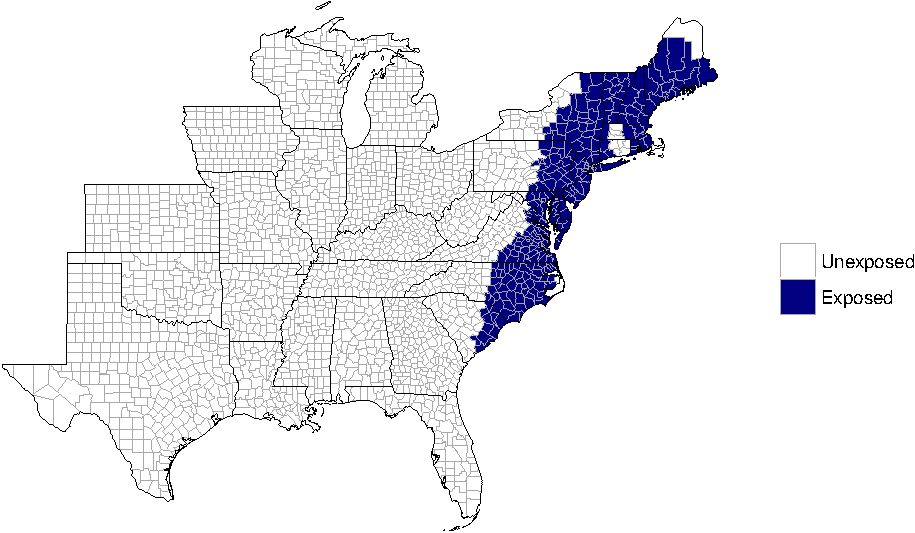
\includegraphics{DraftExposurePaper_files/figure-latex/unnamed-chunk-2-1.pdf}

\section{Discussion}\label{discussion}

\paragraph{Distance-based exposure}\label{distance-based-exposure-1}

There are some sources of uncertainty for storm locations from the best
track hurricane data. These include \ldots{}

However, these best tracks should be fairly reliable for more recent
years of storms, as we use here. Many of the uncertainties related to
storm positions in best track data are more of a concern for the years
before \ldots{} (e.g., pre-19{[}xx{]}).

While there are often several different ``best tracks'' datasets, from
different sources {[}?-- weather services?{]} for other ocean basins,
the ``best tracks'' data from \ldots{}, which is the basis of the tracks
we use here, are the undisputed primary source of tropical storm track
data for the Atlantic basin.

There are a number of limitations to using distance to assess exposure
to tropical storms. Tropical storms vary in size and intensity, and a
measure of distance from the storm track will not incorporate these
differences and so could misclassify exposure both in terms of
generating false positives (counties close to the storm track of very
mild or small-radius storms) and false negatives (e.g., during very
large or intense storms). In particular, the forces of a storm tend to
be distributed around the center in a non-symmetrical way
{[}citation{]}, while distance-based exposure metrics that use buffers
tend to use an equal buffer distance on each side of the storm track
(e.g., {[}citations{]}).

Other distance-based exposure metrics have defined ``exposure'' to occur
only when a storm's center track passes through a county's boundary
(e.g., Zandbergen (2009), who describe this metric of exposure as a
``hit'' on the county). This way of measuring exposure can exclude
nearby counties that suffered extreme conditions from the storm but were
not directly on the hurricane's track, especially since hurricanes can
have a width ({[}typical storm width; citation{]}) that is much larger
than a typical county's width. Further, exposure assessed using this
method has been found to be significantly {[}? double-check{]}
associated with the size and shape of a county (Zandbergen 2009). By
contrast, assessing distance-based exposure based on measuring distance
between the storm track and each county's center would be less
susceptible to differences in county size and shape and so might be a
more reliable metric of exposure than determining if a storm track ever
crossed a county boundary. Further, assessing the minimum distance
between county center and the storm track, as we do here, allows for a
continuous, rather than binary, metric of distance-based exposure to a
storm.

The Zandbergen (2009) study assumed symmetrical activity of storm
related factors,which does not accurately represent storm
characteristics once landfall has been made (Kruk et al. 2010, Halverson
(2015)) {[}GBA-- I did not understand this thought. I agree that storms
are asymmetric, but I don't think that's just after landfall. Is this
something about characteristics of storms as they transform to
extratropical systems? Let's discuss.{]}

There is some uncertainty in the position estimates from the best tracks
hurricane dataset, since the estimation of storm position for best
tracks data involes a poststorm subjective smoothing and integration of
many different types of data (Landsea and Franklin 2013). In a survey of
researchers who perform the poststorm data aggregation to create the
best tracks datasets, uncertainty in the center position of a US
landfalling storm in the ``best tracks'' dataset was estimated at
approximately 8 nautical miles for major hurricanes, 11 nautical miles
for Category 1 and 2 hurricanes, and 15 nautical miles for tropical
storms (Landsea and Franklin 2013). Uncertainty in estimates of a
storm's position also varies by time of day, with more certain estimates
during daylight than during the night (Landsea and Franklin 2013).

Currently, distance parameters involved with assessing risk of a
particular storm have been rather arbitrary, contributing to the
necessity in understanding how such parameters influence a county's
exposure status. In assessing the risk of a given storm based on
distance, recent studies have defined the distance from the storm track
affected by a given storm differently. (Czajkowski, Simmons, and Sutter
2011) assessed county-level risk and exposure based on a three-tierd
definition, with primary counties being those closest to the storm track
on either side, secondary counties being adjacent to primary coutnies,
and tertiary counties adjacent to secondary counties. Such a definition
resulted in an exposure defenition based on an average distance radius
of 120 km on either side of the storm track (Czajkowski, Simmons, and
Sutter 2011). Such a distance is slightly greater than that commonly
used by public health departments (i.e., 100 km) (Czajkowski, Simmons,
and Sutter 2011).

Another study used distance buffers of 30, 60, and 100 kilometers for
different metrics of distance-based exposure (Grabich et al. 2016)
{[}check the paper-- was this distance to any part of a county, or to
the center of the county?{]}.

In a study assessing the association between hurricanes and undesireable
birth outcomes, researchers found that results were not sensitive to the
omission of residences 100 km from the storm path, and that results
varied insignificantly from 30-75 km (Currie and Rossin-Slater 2013).

\paragraph{Rain-based exposure}\label{rain-based-exposure-1}

It can be very difficult to reliably measure rain during extreme rain
events, including tropical storms. For example, a heavy rain can wash
away {[}?{]} rain monitors {[}?{]}. It can also be very hard to measure
rain during heavy wind, as the rain does not fall straight into the
monitor {[}?{]}.

Some of the other possible sources for estimating rain during tropical
storms include \ldots{}{[}Stage IV, TMPA, NEXRAD{]}

The estimated rainfall amounts from our data are likely underestimates.
This data source, however, should be internally consistent and so useful
for comparing across different storms when all exposure estimates are
based on this rain data.

Rainfall estimates are likely underestimates for a few reasons. First,
they are based on averaging hourly measurements to a daily mean
estimate. This averaging would smooth over shorter periods of very
extreme rainfall. Further, this data is averaged over multiple grid
points within each county and so would not fully reflect very extreme
local precipitation (although this might be less of a concern for
classifying exposure to a large-scale storm system, like a tropical
storm, compared to more fine-scale storms). Finally, this NLDAS data
provides a re-analysis that incorporates measured rainfall, using
models, etc., to incorporate that observed data into a spatially and
temporally continuous dataset of rainfall. However, during extreme
storms, the problems with measuring rainfall using {[}rain monitors{]}
would propogate into the NLDAS data, so although NLDAS would prevent
missing values during the storm if monitors are not able to provide
data, if monitors are out, rainfall estimates from NLDAS will be based
more on models than on observations. More on NLDAS bias low here
(Villarini et al. 2011). Such bias, though unimportant in our analysis,
may play a larger role in the extrapolation to other studies or exposure
analysese where the precipitation cutoffs used here may provide a
threshold that results in the missclassification of less affected
counties as exposed.

Exposure classification based on rainfall has some advantages. For
example, it allows the identification of exposed counties that are
inland, rather than coastal, but that were affected by heavy rainfall
during the storm. Often, storm-related deaths are associated with inland
flooding. In fact, over half of the hurricane-related fatalities from
1970 to 1999 were a result of freshwater flooding, accounting for the
vast majority of deaths in inland counties (Rappaport 2000). In another
analysis, researchers found that 79\% of freshwater-drowning fatalities
occured in inland counties,(Czajkowski, Simmons, and Sutter 2011)
further stressing the importance of rainfall in hurricane risk analysis.
Storms can produce a lot of rain especially in certain topographies,
like near mountains, so counties that are well inland can sometimes
experience more extreme rain that other counties at similar distances
from the storm's track.

In comparison to the storm track, the areas of extreme rain and extreme
wind can vary. For example, storms undergoing an extratropical
transition can bring heavy rains to the left of the storm's center
track, while extreme winds are more common to the right of the track
(Halverson 2015, Grabich et al. (2016) GBA-- I think it would be better
to just use meteorological papers as references for this point. The
Halverson paper is great, but the Grabich paper I think might just be a
secondary, rather than primary, reference for this point, so I think we
could probably find a more direct reference). Wind speeds are typically
more severe to the right of the storm's track because here the
counter-clockwise cyclonic {[}right word?{]} winds are moving in the
same direction as the forward motion of the storm, creating an additive
effect for total windspeeds {[}citation{]}. In contrast, rains can be
heaviest to the left of the storm's track, especially in cases when the
storm interacts with a downstream ridge (Atallah, Bosart, and Aiyyer
2007).

Some storms can be of lower intensity (i.e., on the Saffir-Simpson
scale) yet bring dangerous rainfall, including well inland of the
storm's landfall. For example, storms including Floyd in 1999, Gaston in
2004, Irene in 2011, and Lee in 2011, have had severe inland impacts,
often through extreme rainfall, as post-tropical storms (Halverson
2015). This rainfall can be particularly severe in the Appalachians
(Halverson 2015). Further, heavier rainfall is more common for storms
moving at slower forward speeds (Chang, Yang, and Kuo 2013). Storms with
a slower forward speed and larger rainfall area contribute to a longer
duration of rainfall, and therefore an increased chance of flood-related
damage (Rezapour and Baldock 2014).

For example,

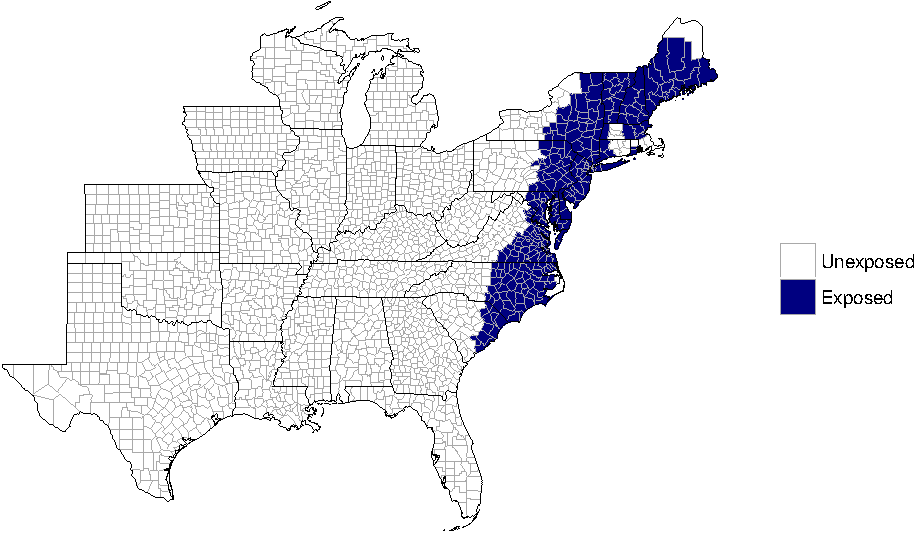
\includegraphics{DraftExposurePaper_files/figure-latex/unnamed-chunk-3-1.pdf}

\paragraph{Wind-based exposure}\label{wind-based-exposure-1}

Wind suffers from similar challenges for measuring during tropical
storms. In particular, the strong winds of tropical storms can break or
blow away the anemometers used to measure wind speed.

Here, we used wind speed models, rather than observed wind speed, to
estimate exposure to tropical storms based on winds.

A variety of other wind speed models exist besides the one used here. In
particular, there are options for wind speed models as far as \ldots{}
One study used a very simple model of constant winds up to a distance of
30 km from the storm track and a simple model of wind decay beyond that
distance (Zandbergen 2009), based on a model developed by \ldots{}
{[}see references for this paper{]}. Another study used wind data from a
NOAA public database based on real-time hurricane wind analysis, rather
than modeling windspeeds themselves (Grabich et al. 2016) {[}see the
Powell reference in this paper for more on that data{]}.

There is some uncertainty in the maximum wind speed values estimated at
each synoptic time for each storm. For US landfalling storms, the
estimate of storm intensity in the best tracks dataset is estimated to
have an uncertainty of around 8 knots for tropical storms, 10 knots for
Category 1 and 2 hurricanes, and 13 knots for major hurricanes (Landsea
and Franklin 2013). Since the wind model used here uses these best
tracks maximum wind speeds as an input, this uncertaintly would
propogate into our estimates of windspeed within each county for each
storm.

A recent study suggests that nearly all states east of the Rocky
Mountains have experienced wind exposure associated with either tropical
or post-tropical storms (Kruk et al. 2010).

Exposure metrics based on wind speed may not provide an accurate
representation of the communities exposed to a given storm, since, while
wind speeds rapidly decay after landfall {[}citation{]}, extreme rain
can persist,for some storms affecting a large number of inland counties,
which would be underrepresented using an exposure metric the depends on
windspeed.

Examples of studies that used windspeed as a sole criteria when
determining tropical storm exposure include \ldots{} {[}citation{]}. In
other studies, wind criteria have been combined with distance criteria,
and with windspeed modeled based on maximum sustained windspeed
estimates at each ``best tracks'' observation, combined with a simple
model of decay in wind speed at distances further from the storm's
center (wind speed equals the storm's maximum sustained windspeed up to
30 kilometers from the storm's center then follows a simple decay
function beyond that distance) (Zandbergen 2009) {[}GBA-- this paper
references another paper with more details on this decay model for
windspeed-- the Gray and Klotzbach reference they have{]}. In this
study, wind speed cutoffs of 40 mph, 75 mph, and 115 mph were used to
determine if a county was exposed to a storm (tropical, hurricane-force,
and intense hurricane-force, respectively) (Zandbergen 2009).

One study found that using a distance-based exposure metric that
required the storm track to cross a county boundary assessed a number of
counties as ``unexposed'' that suffered tropical storm- or
hurricane-force winds from the storm and were assessed as ``exposed''
using a metric that combined distance and windspeed (Zandbergen 2009);
in fact, almost twice as many counties were assessed as having been
exposed to at least one tropical storm between 1851 and 2003 when
exposure was determined based on a combined wind-distance metric
compared to a ``hit'' distance-based metric (Zandbergen 2009). This
suggests that some distance-based metrics might result in a number of
false negatives for county-level storm exposure.

Studies that have used wind-based exposure metrics have used a variety
of windspeed cutoff values to determine exposure. One study, for
example, assigned a binary exposure value based on windspeed thresholds
of 63 and 119 kilometers per hour, as well as a continuous exposure
metric based on the exact value of the windspeed in the county during
the storm and a categorical exposure metric based on the Saffir-Simpson
storm severity categories (Grabich et al. 2016).

\paragraph{Other ways of assessing tropical storm
exposure}\label{other-ways-of-assessing-tropical-storm-exposure}

One study used FEMA disaster declarations as a binary indicator of
tropical storm exposure (Grabich et al. 2016). They found that this
metric tended to assess a lot more counties as ``exposed'' to a storm
than distance- or wind-based metrics (Grabich et al. 2016), although
they only compared the two exposure metrics as applied to four storms
(Hurricanes Charley, Frances, Ivan, and Jeanne in Florida in 2004).

\paragraph{Example uses of exposure
datasets}\label{example-uses-of-exposure-datasets}

\paragraph{Table including various exposure papers and the parameters
used}\label{table-including-various-exposure-papers-and-the-parameters-used}

\section*{References}\label{references}
\addcontentsline{toc}{section}{References}

\hypertarget{refs}{}
\hypertarget{ref-Atallah2007}{}
Atallah, Eyad, Lance F. Bosart, and Anantha R. Aiyyer. 2007.
``Precipitation Distribution Associated with Landfalling Tropical
Cyclones over the Eastern United States.'' \emph{Monthly Weather Review}
135: 2185--2206.
doi:\href{https://doi.org/10.1175/MWR3382.1}{10.1175/MWR3382.1}.

\hypertarget{ref-Chang2013}{}
Chang, Chih-Pei, Yi-Ting Yang, and Hung-Chi Kuo. 2013. ``Large
Increasing Trend of Tropical Cyclone Rainfall in Taiwan and the Roles of
Terrain.'' \emph{Journal of Climate} 26: 4136--47.
doi:\href{https://doi.org/10.1175/JCLI-D-12-00463.1}{10.1175/JCLI-D-12-00463.1}.

\hypertarget{ref-Currie2013}{}
Currie, Janet, and Maya Rossin-Slater. 2013. ``Weathering the Storm:
Hurricanes and Birth Outcomes.'' \emph{Journal of Health Economics} 32:
487--503.
doi:\href{https://doi.org/10.1016/j.jhealeco.2013.01.004}{10.1016/j.jhealeco.2013.01.004}.

\hypertarget{ref-Czajkowski2011}{}
Czajkowski, Jeffrey, Kevin Simmons, and Daniel Sutter. 2011. ``An
Analysis of Coastal and Inland Fatalities in Landfalling US
Hurricanes.'' \emph{Natural Hazards} 59: 1513--31.
doi:\href{https://doi.org/10.1007/s11069-011-9849-x}{10.1007/s11069-011-9849-x}.

\hypertarget{ref-Grabich2016}{}
Grabich, S. C., J. Horney, C. Konrad, and D. T. Lobdell. 2016.
``Measuring the Storm: Methods of Quantifying Hurricane Exposure with
Pregnancy Outcomes.'' \emph{Natural Hazards Review} 17 (1):
06015002--1--06015002--7.
doi:\href{https://doi.org/10.1061/(ASCE)NH.1527-6996.0000204}{10.1061/(ASCE)NH.1527-6996.0000204}.

\hypertarget{ref-Halverson2015}{}
Halverson, Jeffrey B. 2015. ``Second Wind: The Deadly and Destructive
Inland Phase of East Coast Hurricanes.'' \emph{Weatherwise} 68 (2):
20--27.
doi:\href{https://doi.org/10.1080/00431672.2015.997562}{10.1080/00431672.2015.997562}.

\hypertarget{ref-Kruk2010}{}
Kruk, Michael C., Ethan J. Gibney, David H. Levinson, and Michael
Squires. 2010. ``A Climatology of Inland Winds from Tropical Cyclones
for the Eastern United States.'' \emph{Journal of Applied Meteorology
and Climatology} 49: 1538--47.
doi:\href{https://doi.org/10.1175/2010JAMC2389.1}{10.1175/2010JAMC2389.1}.

\hypertarget{ref-Landsea2013}{}
Landsea, Christopher W., and James L. Franklin. 2013. ``Atlantic
Hurricane Database Uncertainty and Presentation of a New Database
Format.'' \emph{Monthly Weather Review} 141: 3576--92.

\hypertarget{ref-Levinson2010}{}
Levinson, David H., Howard J. Diamond, Kenneth R. Knapp, Michael C.
Kruk, and Ethan J. Gibney. 2010. ``Toward a Homogenous Global Tropical
Cyclone Best-Track Dataset.'' \emph{American Meteorological Society} x:
377--80.
doi:\href{https://doi.org/10.1175/2010BAMS2930.1}{10.1175/2010BAMS2930.1}.

\hypertarget{ref-Lin2005}{}
Lin, Ying, and Kenneth E. Mitchell. 2005. ``The NCEP Stage II/IV Hourly
Precipitation Analyses: Development and Applications.'' \emph{19th
Conference of Hydrology, American Meteorlogical Society}.

\hypertarget{ref-Rappaport2000}{}
Rappaport, Edward N. 2000. ``Loss of Life in the United States
Associated with Recent Atlantic Tropical Cyclones.'' \emph{Bulletin of
the American Meteorological Society} x: 2065--73.

\hypertarget{ref-Rezapour2014}{}
Rezapour, Mehdi, and Tom E. Baldock. 2014. ``Classification of Hurricane
Hazards: The Importance of Rainfall.'' \emph{Weather and Forcasting} 29:
1319--31.

\hypertarget{ref-Villarini2011}{}
Villarini, Gabriele, James A. Smith, Mary Lynn Baeck, Timothy Marchok,
and Gabriel A. Vecchi. 2011. ``Characterization of Rainfall Distribution
and Flooding Associated with U.S. Landfalling Tropical Cyclones:
Analysis of Hurricanes Frances, Ivan, and Jeanne (2004).'' \emph{Journal
of Geophysical Research} 116: D23116.

\hypertarget{ref-Zandbergen2009}{}
Zandbergen, Paul A. 2009. ``Exposure of US Counties to Atlantic Tropical
Storms and Hurricanes, 1851--2003.'' \emph{Natural Hazards} 48: 83--99.
doi:\href{https://doi.org/10.1007/s11069-008-9250-6}{10.1007/s11069-008-9250-6}.

\end{document}


